\documentclass[aspectratio=169]{beamer}              % only frames

% for themes, etc.
\mode<presentation>
\usetheme{Madrid} 
\usecolortheme{crane}

%\usepackage{times}  % fonts are up to you
% The usual suspects
\usepackage{multirow, booktabs, dcolumn, color, graphicx} % Tables\usepackage{graphicx}
\usepackage{amsmath,amssymb,amsthm}
% Strikethrough text
\usepackage{soul}
% Adjust box to fit tabulars
\usepackage{adjustbox}
% Embed video
\usepackage{media9}
% For notes
\usepackage{pgfpages}
%\setbeameroption{hide notes} % Only slides
%\setbeameroption{show only notes} % Only notes
\setbeameroption{hide notes} % Both
% Give a slight yellow tint to the notes page
%\setbeamertemplate{note page}{\pagecolor{yellow!5}\insertnote}\usepackage{palatino}
% Use colors by name
\usepackage{xcolor}
% EMBEDDING VIDEO IS POSSIBLE WITH PDFPC USE PDF PC to present
\usepackage{multimedia}



% The table highlighting for hypothesis discussion.
\usepackage[beamer,customcolors]{hf-tikz}
\usetikzlibrary{calc}

% To use background images
\newenvironment{colorframe}[2][]{%
\setbeamercolor{background canvas}{bg=#1}
\begin{frame}\color{white}}
{\end{frame}}


% To set the hypothesis highlighting boxes red.
\tikzset{hl/.style={
    set fill color=red!80!black!40,
    set border color=red!80!black,
  },
}

% Set Graphics folder
\graphicspath{{./figures/}}


% these will be used later in the title page
\title{Computer Networks}
\subtitle{Routing and Its Woes}
\author{Irfan Kanat}
\institute[CBS]{{Department of Digitization}\\ Copenhagen Business School}
\date{\today}



\begin{document}

% this prints title, author etc. info from above
\begin{frame}

	\titlepage

\end{frame}

\note{We will talk about how routing can be exploited for fun and profit.

}



\begin{colorframe}[black]

	\centering
	\Large
	Can you think of a misuse of routing algorithms?

\end{colorframe}

{
\usebackgroundtemplate{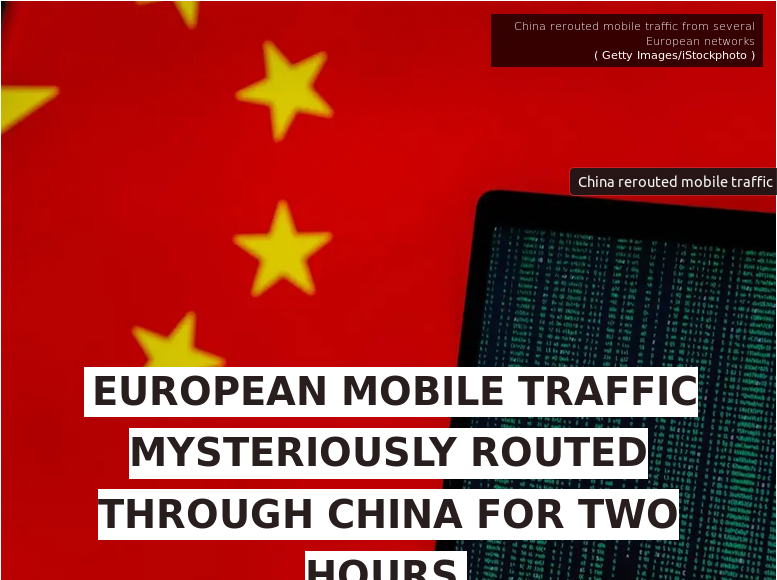
\includegraphics[width=\paperwidth,height=\paperheight]{figures/BGPAttack.png}}%
	\begin{frame}
	\frametitle{}



	\end{frame}
}


\note{In June 2019, European internet traffic was routed through China (also in 2010). 

This can allow interception of data, or MITM attacks.

Similar attacks happened in the past as well.

They rely on manipulating BGP.

}

\begin{frame}
	\frametitle{Lag and Package Loss}
    
    \includegraphics<1>[width = \textwidth, height = .85\textheight, keepaspectratio]{figures/Lag.png}
	\includegraphics<2>[width = \textwidth, height = .85\textheight, keepaspectratio]{figures/lagAndCo.png}

\end{frame}

\begin{frame}
	\frametitle{DDOS: Weaponized Package Loss}
    
    \movie{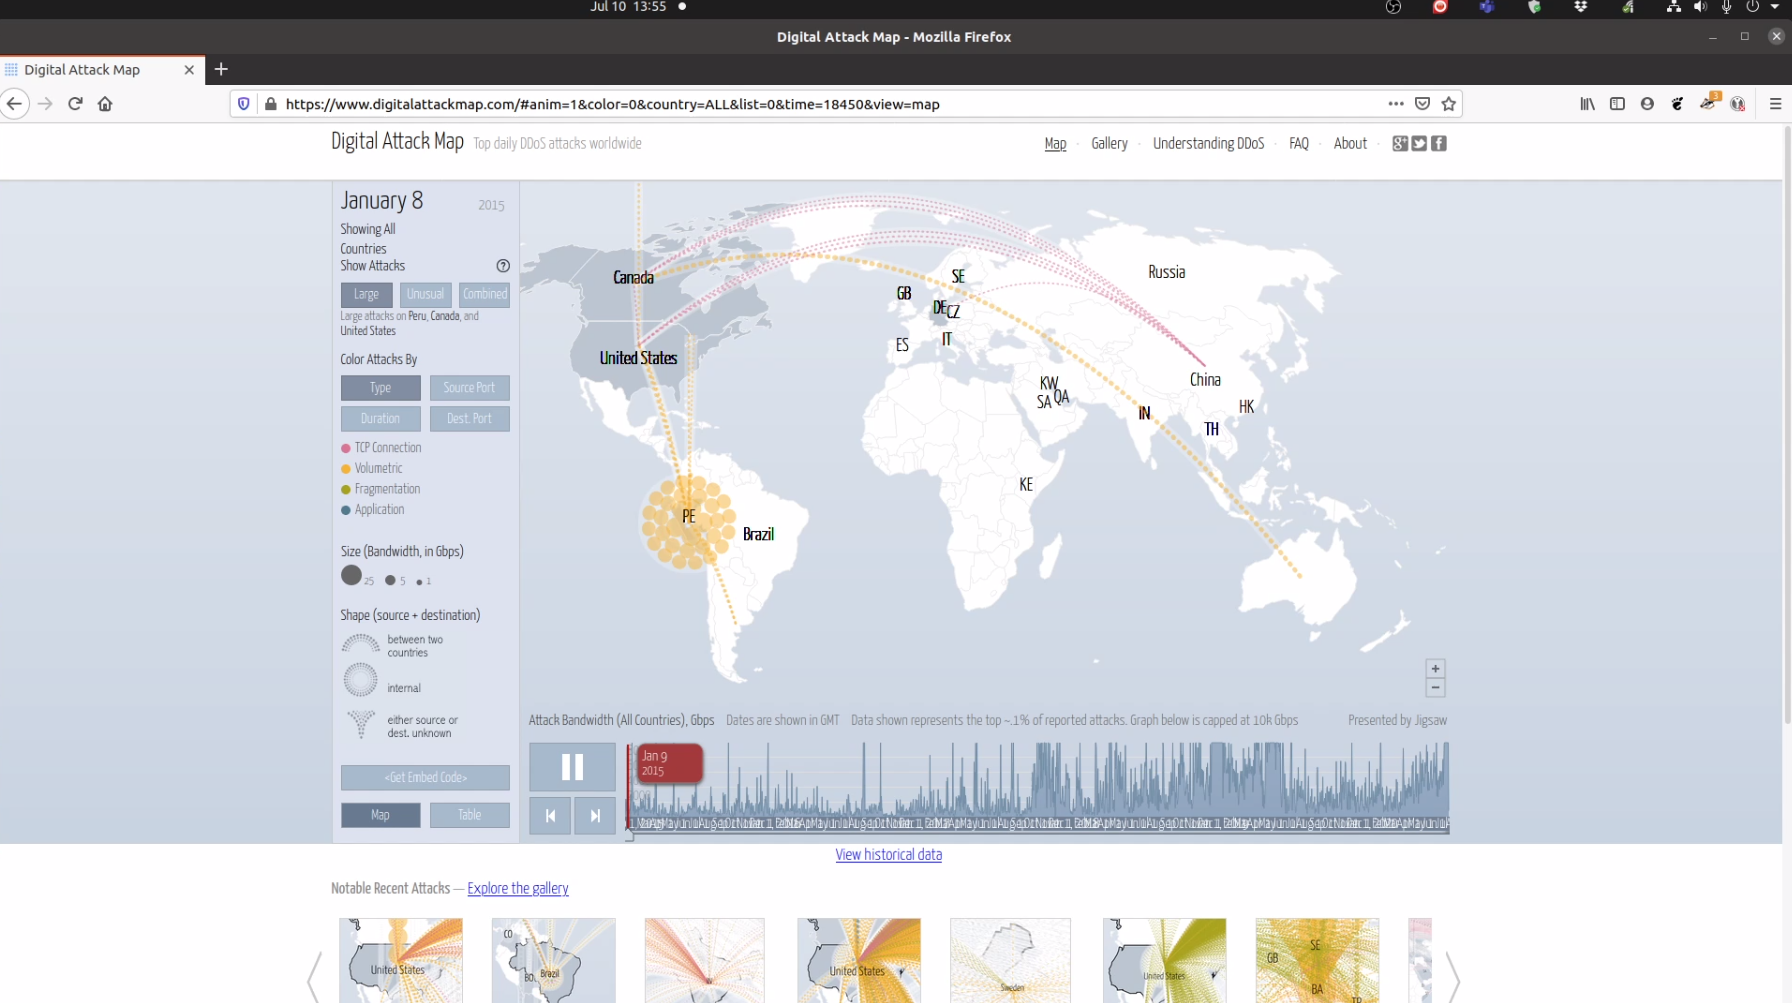
\includegraphics[width = \textwidth]{figures/ddos.png}}{figures/ddos.mp4}

\end{frame}


\begin{frame}
	\frametitle{Networking and Security: Segmentation}

	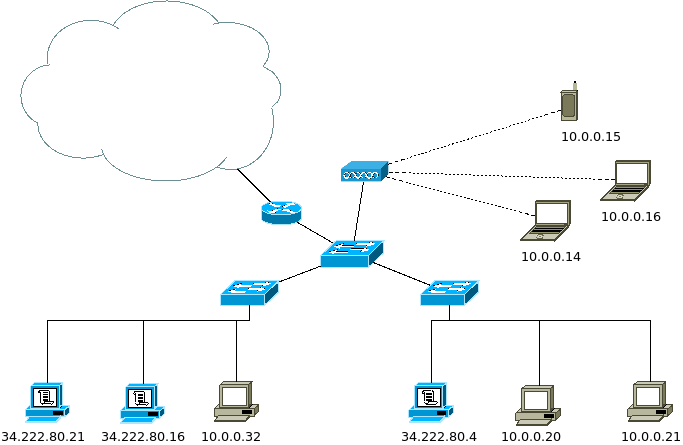
\includegraphics[width = \textwidth, height = .85\textheight, keepaspectratio]{figures/Segmentation.png}

\end{frame}

\note{
	Segmentation: it kept coming up in cases we read (target esp.)

	The idea is, you can have multiple virtual networks on the same hardware. So you put your customer facing machines on one network, and your back office oprations in another, and perhaps mission critical systems on yet another network. What this means is they all get their own IP prefix and treat each other as nodes in different networks.

}


\begin{frame}
	\frametitle{Zero Trust Architecture}

	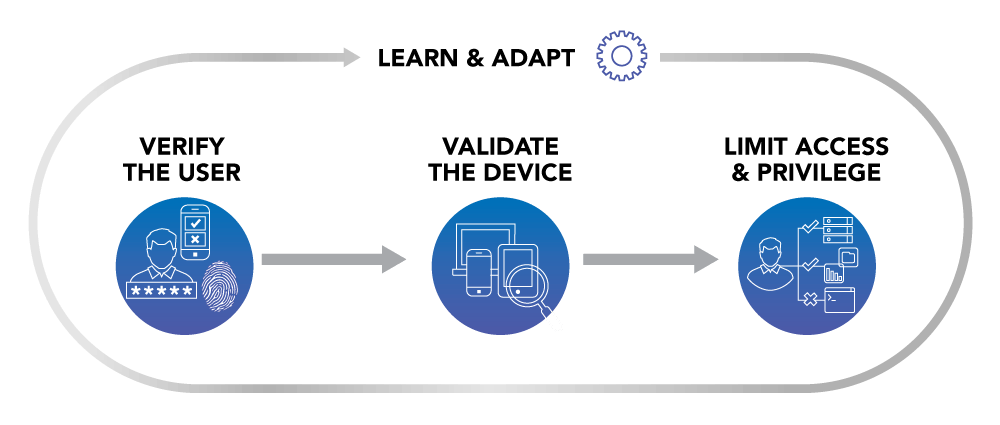
\includegraphics[width = \textwidth, height = .85\textheight, keepaspectratio]{figures/zero-trust-cycle-diagram.png}

\end{frame}

\note{This is a more recent trend.

No trust is granted based on network location.

All devices and users authenticated 

Data released on a need to know basis     

Focus is on protecting resources and not network segments.

This is in contrast to prior approaches that focused on network segments.

NIST draft 800-207
}



\begin{frame}
	\frametitle{Intrusion Detection on Networks}

	Unusual behavior on your network \vspace{1em}

	Heuristics \vspace{1em}

	Known signatures

\end{frame}

\note{
A few examples:

A client is rapidly sending packages to a large number of ip's and ports (proably nmap scan)

A server with minimal functionality generally does not initiate exchanges. Meaning TCP syn packets do not generally originate from servers. If you see your server reaching out.

Or generating traffic on ports it is not supposed to generate traffic on...

Then you know that there is something wrong.

Attacks often have certain characteristics. These attack specific characteristics are called signatures. These signatures are often shared through intel sharing schemes. If your network demonstrates behavior that matches the signature IDS will pick up.
}

\begin{frame}
\frametitle{NIDS Solutions}

	\begin{columns}
		\begin{column}{0.5\textwidth}

			Appliances \vspace{1em}

			Software
	
		\end{column}

		\begin{column}{0.5\textwidth}

			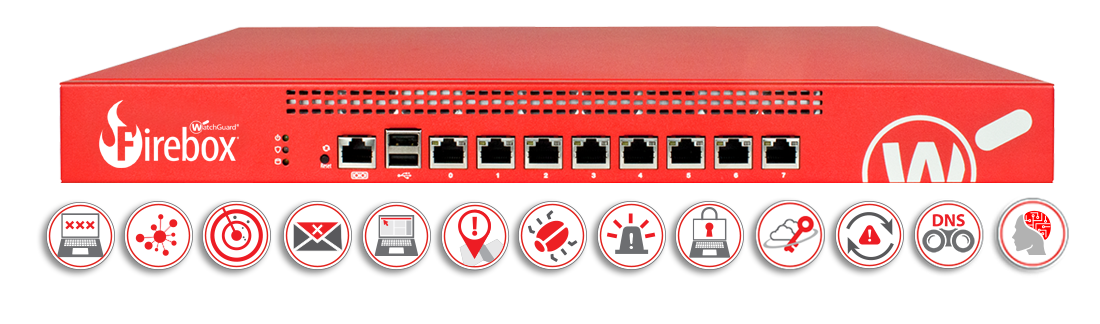
\includegraphics[width = \textwidth, height = .85\textheight, keepaspectratio]{figures/nids.png}

		\end{column}

	\end{columns}

\end{frame}


\note{
IDS can be provided by appliances (like Watchguard), or by software solution (like SNORT).

Appliances are used for larger networks where latency can be an issue.

The network based intrusion detection is often coupled with end point ids. That is not within our scope today.}




\end{document}
